We recall the definition of morphism weight and object weight relative to a type graph~\cite{endrullis2024generalized_icgt}.

\begin{notation}[\cite{endrullis2024generalized_arxiv_v2}]
Let \(A,B,C\) be objects. For morphism $\alpha\mathop{\colon} A \mathop{\to} B$, we introduce the notation 
          $$\set{ \alpha \mathop{\star} - \mathop{=} \gamma } \overset{\operatorname{def}}{=} \{ \beta \mathop{\in} \operatorname{Hom}(B, C) \mathop{\mid} \alpha \mathop{\star} \beta \mathop{=} \gamma \}.$$ 
For morphism $\beta\mathop{\colon} B \mathop{\to} C$, we introduce the notation
          $$\set{ - \mathop{\star} \beta \mathop{=} \gamma }  \overset{\operatorname{def}}{=} \{ \alpha \mathop{\in} \operatorname{Hom}(A, B) \mathop{\mid} \alpha \mathop{\star} \beta \mathop{=} \gamma \}.$$
For morphism set $E \mathop{\subseteq} \operatorname{Hom}(A,B)$ and morphism $\beta\mathop{\colon} B \mathop{\to} C$, we introduce the notation
          $$E \mathop{\star} \beta \overset{\operatorname{def}}{=} \set{ \alpha \mathop{\star} \beta \mathop{\mid} \alpha \mathop{\in} E }.$$
\end{notation}
Analogous to measuring a physical object, a morphism ruler measures a morphism as follows.
\begin{definition} 
    \label{def:measurement_of_a_morphism_relative_to_a_morphism_ruler}
    The \emph{measurement} of a morphism \( h:G \mathop{\to} T \) relative to a morphism-ruler \( e: X \mathop{\to} T \), denoted by $m_e(h)$, is defined as:
                \(
                m_e(h) 
                    \overset{\operatorname{def}}{=}
                \card{\{- \mathop{\star} h \mathop{=} e\}}.
                \)
\end{definition}


Combining the measurements of a morphism provided by all morphism-rulers with the help of a weight function $w$ gives the weight of the morphism (Definition~\ref{def:weight_of_a_morphism_relative_to_a_type_graph}).
\begin{definition} 
    \label{def:weight_of_a_morphism_relative_to_a_type_graph}
        Let $\mathcal{T}=(T,\mathbb{E},\mathcal{S},w)$ be a finitary weighted type graph.
         The \textbf{weight of a morphism $h: G \mathop{\rightarrow} T$ relative to a type graph $\mathcal{T}$}\index{Weight of a morphism!of the type graph method} is defined as the semiring product of $w(e)^{m_e(h)}$ for all $e \mathop{\in} \mathbb{E}$:
        \[  w_{\mathcal{T}}(h) \overset{\operatorname{def}}{=} \underset{e \mathop{\in} \mathbb{E}}{\mathop{\bigodot}} 
                w(e)^{m_e(h)}.\]
\end{definition}
Finally, the weight of an object is defined as the semiring sum of the weights of all morphisms from the object to the underlying type graph $T$ of the weighted type graph $\mathcal{T}$.
\begin{definition}[Object weight]
    \label{def:weight_of_an_object_relative_to_a_type_graph}
       Let $\mathcal{T}=(T,\mathbb{E},\mathcal{S},w)$ be a finitary weighted type graph. The \textbf{weight of an object \( G \)}\index{Weight of an object!of the type graph method} is defined as the semiring sum of $w_\mathcal{T}(h)$, for all \( h \mathop{\in} \operatorname{Hom}(G,T) \):
        \[ w_\mathcal{T}(G) \overset{\operatorname{def}}{=} \underset{h \mathop{\in} \operatorname{Hom}(G,T)}{\mathop{\bigoplus}}  w_\mathcal{T}(h). \]
\end{definition}

\begin{example}
    Consider the two morphisms shown below
    %  Figure~\ref{fig:example:two_weighted_type_graph_morphisms}
    % \begin{figure}[H]
    %     \centering
    \begin{center}
        \begin{tikzpicture}
          \graphbox{\( L \)}{-50mm}{0mm}{40mm}{39mm}{2mm}{-10mm}{
            \coordinate (o) at (0mm,-10mm); 
            \node[draw,circle] (l1) at ($(o)+(-10mm,0mm)$) {1};
            \node[draw,circle] (l2) at ($(l1)+(2,0)$) {2};
            \node[draw,circle] (l3) at ($(l1)+(1,0)$) {3};
            \draw[] (l1) -- (l3) node[midway,above] {$a$};
            \draw[] (l3) -- (l2) node[midway,above] {$a$};
        } 
            \graphbox{$T$}{0mm}{0mm}{40mm}{39mm}{-10mm}{-20mm}{
                \node[draw,circle] (1) at (0,0) {$1\ 2$};
                \node[draw,circle] (2) at (2,0) {3};
                \draw[->] (1) edge[loop above] node[midway, above] {$a^{1}$} (1) ;
                \draw[->] (1) edge[loop below] node[midway, below] {$b^{1}$} (1) ;
                \draw[->] (1) edge[bend left] node[midway, above] {$a^{1}$}  (2)  ;
                \draw[->] (2) edge[bend left] node[midway, below] {$a^{1}$} (1)   ;
            }
            \node () at (-5mm,-15mm) {$\overset{h_{11}^1}{\to}$};
        \end{tikzpicture}

        \vspace{2mm}
            \begin{tikzpicture}
              \graphbox{\(L\)}{-50mm}{0mm}{40mm}{39mm}{2mm}{-7mm}{
                \coordinate (o) at (0mm,-10mm); 
                \node[draw,circle] (l1) at ($(o)+(-10mm,0mm)$) {1};
                \node[draw,circle] (l2) at ($(l1)+(2,0)$) {2};
                \node[draw,circle] (l3) at ($(l1)+(1,0)$) {3};
                \draw[] (l1) -- (l3) node[midway,above] {$a$};
                \draw[] (l3) -- (l2) node[midway,above] {$a$};
            } 
                \graphbox{$T$}{0mm}{0mm}{40mm}{39mm}{-10mm}{-20mm}{
                    \node[draw,circle] (1) at (0,0) {$1\ 2\ 3$};
                    \node[draw,circle] (2) at (2,0) {};
                    \draw[->] (1) edge[loop above] node[midway, above] {$a^{1}$} (1) ;
                    \draw[->] (1) edge[loop below] node[midway, below] {$b^{1}$} (1) ;
                    \draw[->] (1) edge[bend left] node[midway, above] {$a^{1}$}  (2)  ;
                    \draw[->] (2) edge[bend left] node[midway, below] {$a^{1}$} (1)   ;(1)   ;
                }
                \node () at (-5mm,-15mm) {$\overset{h_{11}^2}{\to}$};
            \end{tikzpicture}
    \end{center}
       and the weighted type graph shown 
       below 
    \begin{center}
        % \resizebox{0.5\textwidth}{!}{
        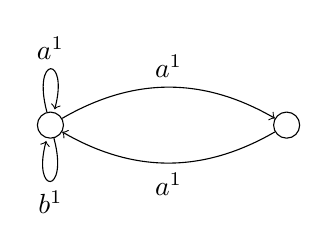
\begin{tikzpicture}
            [scale=1.5]
            \graphbox{}{0mm}{0mm}{32mm}{24mm}{-10mm}{-12mm}{
                \node[draw,circle] (1) at (0,0) {};
                \node[draw,circle] (2) at (2,0) {};
                \draw[->] (1) edge[loop above] node[midway, above] {$a^{1}$} (1) ;
                \draw[->] (1) edge[loop below] node[midway, below] {$b^{1}$} (1) ;
                \draw[->] (1) edge[bend left] node[midway, above] {$a^{1}$}  (2)  ;
                \draw[->] (2) edge[bend left] node[midway, below] {$a^{1}$} (1)   ;
            }
        \end{tikzpicture}
        % } 
    \end{center}
    We have \begin{itemize}
        \item $ w_\mathcal{T}(h_{11}^1) \mathop{=} w(e_{13a})^{m_{e_{13a}}(h_{11}^1)} \mathop{\odot} w(e_{31a})^{m_{e_{31a}}(h_{11}^1)} =
     1^1 * 1^1 \mathop{=} 1$,
        \item $
        w_\mathcal{T}(h_{11}^2) 
        % \mathop{=} 1^1 * 1^1 
        \mathop{=} 1$.
    \end{itemize}
\end{example}   
